\documentclass[crop,tikz]{standalone}% 'crop' is the default for v1.0, before it was 'preview'
%\usetikzlibrary{...}% tikz package already loaded by 'tikz' option
\begin{document}

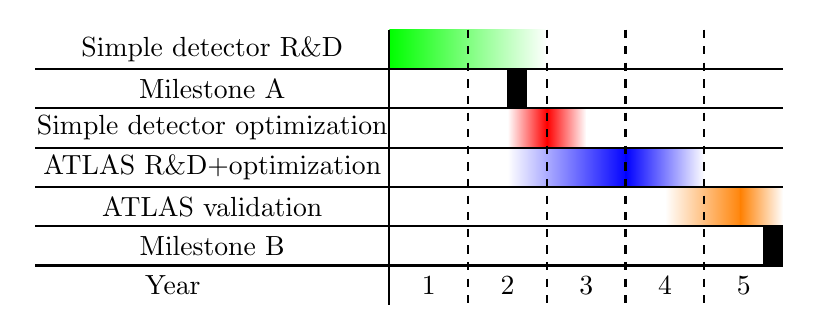
\begin{tikzpicture}[scale=.5]
  \shade[left color=green, right color=white](0,0) rectangle (4.,-1);

  \fill[color=black](3.,-1) rectangle (3.5,-2);
      
    \shade[left color= white,right color=red](3,-2) rectangle (4.,-3);
    \shade[left color=red,right color=white](4.,-2) rectangle (5.,-3);


    \shade[left color=white, right color=blue](3,-3) rectangle (6.05,-4);
    \shade[left color=blue,right color=white](6,-3) rectangle (8,-4);

    %\fill[color=black](7.5,-4) rectangle (8,-5);

    \shade[left color = white, right color=orange](7.,-4) rectangle (9,-5);
    \shade[left color=orange,right color=white](8.9,-4) rectangle (10,-5);

    \fill[color=black](9.5,-5) rectangle (10,-6);

    \node at (-4.5,-0.5) { Simple detector R\&D};
    \node at (-4.5,-1.5) { Milestone A}; % make a choice on algorithm to develop
    \node at (-4.5,-2.5) { Simple detector optimization};
    \node at (-4.5,-3.5) { ATLAS R\&D+optimization};
    \node at (-4.5,-4.5) { ATLAS validation};
    \node at (-4.5,-5.5) { Milestone B}; % Use in ATLAS
    \node at (-5.5,-6.5) { Year}; % Use in ATLAS
    \node at (1,-6.5)  {1};
    \node at (3,-6.5)  {2};
    \node at (5,-6.5)  {3};
    \node at (7,-6.5)  {4};
    \node at (9,-6.5)  {5};
    \draw[thick](0,0) -- (0,-7);
    \draw[dashed, thick](2,0) -- (2,-7);
    \draw[dashed, thick](4,0) -- (4,-7);
    \draw[dashed, thick](6,0) -- (6,-7);
    \draw[dashed, thick](8,0) -- (8,-7);

    \draw[thick](-9,-1) -- (10,-1);
    \draw[thick](-9,-2) -- (10,-2);
    \draw[thick](-9,-3) -- (10,-3);
    \draw[thick](-9,-4) -- (10,-4);
    \draw[thick](-9,-5) -- (10,-5);
    \draw[very thick](-9,-6) -- (10,-6);
    %\draw[thick](-9,-7) -- (10,-7);

\end{tikzpicture}
\end{document}